
\documentclass[12pt,letterpaper]{report}
\usepackage[numbers,sort&compress]{natbib}
\usepackage[letterpaper]{geometry}
\usepackage{fancyhdr}
\usepackage{afterpage}
\usepackage{graphicx}
\usepackage{amsmath,amssymb,amsbsy}
\usepackage{dcolumn,array}
\usepackage{tocloft}
\usepackage{asudis}
\usepackage{indentfirst}
\usepackage{listings}
\usepackage{multirow,booktabs,caption}
\usepackage{xfp}
\usepackage{pgfplots}
\usepackage{xcolor}
\usepackage{tikz}
\usepackage{subcaption}
\usepackage{minted}
\usepackage{pdfpages}
\usepackage{threeparttable}

%-- Customizing
\PassOptionsToPackage{hyphens}{url}\usepackage[hidelinks]{hyperref}

\def\code#1{\texttt{#1}}

\graphicspath{ {./images/} }

\makeatletter
    \def\maxwidth#1{
        \ifdim
            \Gin@nat@width>#1 #1
        \else                
            \Gin@nat@width
        \fi}
\makeatother

\newcommand*{\image}[4]{
  \begin{figure}[tb]
    \begin{center}
      \includegraphics[width=0.8\maxwidth{\textwidth}]{#1}
      \caption{#2}
      \label{#3}
    \end{center}
  \end{figure}}


\DeclareCaptionLabelSeparator*{spaced}{\\[2ex]}
\captionsetup[table]{textfont=it,format=plain,justification=justified,
  singlelinecheck=false,labelsep=spaced,skip=0pt}
\captionsetup[figure]{labelsep=period,labelfont=it,justification=justified,
  singlelinecheck=false,font=doublespacing}


\begin{document}
%-----------------------front matter
\pagenumbering{roman}
\title{Visualizing Information Flow\\ \ \\
Graph-Based Approach to Tracing Data Dependencies for Binary Analysis}
\author{Bailey Capuano}
\degreeName{Master of Science}
\defensemonth{April}
\gradmonth{May}
\gradyear{2022}
\chair{Yan Shoshitaishvili, Co-Chair \\ Ruoyu Wang, Co-Chair \\ Adam Doup\'e}		
\maketitle
\doublespace
\begin{abstract}
Binary analysis and software debugging are critical tools in the modern software security ecosystem. With the security arms race between attackers discovering and exploiting vulnerabilities and the development teams patching bugs ever-tightening, there is an immense need for more tooling to streamline the  binary analysis and debugging processes. Whether attempting to find the root cause for a buffer overflow or a segmentation fault, the analysis process often involves manually tracing the movement of data throughout a program's life cycle. Up until this point, there has not been a viable solution to the human limitation of maintaining a cohesive mental image of the intricacies of a program's data flow. 

This thesis proposes a novel data dependency graph (DDG) analysis as an addition to \code{angr}'s analyses suite. This new analysis ingests a symbolic execution trace in order to generate a directed acyclic graph of the program's data dependencies. In addition to the development of the backend logic needed to generate this graph, an \code{angr management} view to visualize the DDG was implemented. This user interface provides functionality for ancestor and descendant dependency tracing and sub-graph creation. To evaluate the analysis, a user study was conducted to measure the view's efficacy in regard to binary analysis and software debugging. The study consisted of a control group and experimental group attempting to solve a series of 3 challenges and subsequently providing feedback concerning perceived functionality and comprehensibility pertaining to the view. 

The results show that the view had a positive trend in relation to challenge-solving accuracy in its target domain, as participants solved 32\% more challenges 21\% faster when using the analysis than when using vanilla \code{angr management}.
\end{abstract}
\dedicationpage{\\Thank you to my girlfriend McKenna for her unwavering support and unique ability to ground me when the tasks and deadlines seemed insurmountable. Thank you for being my rock. I am so incredibly lucky to have you by my side, Forvie.}
\acknowledgementpage{\\ Thank you to Adam for his invaluable support throughout this process and for sparking within me an initial passion for cybersecurity. His undergraduate information assurance course was my first real introduction to the field and, from the first assignment that had us finding ways to crash other students’ programs, I was absolutely hooked. 
\linebreak
\linebreak
I would like to thank Fish for his guidance and for putting up with my incessant Discord and Slack pings asking for programming advice as I attempted to navigate angr's codebase. No matter the question, he would somehow always have the answer. 
\linebreak
\linebreak
Lastly, I would like to thank Yan for taking me under his guidance for this thesis and for providing me a wealth of opportunities to further hone my passion for binary analysis through his fantastic courses in computer systems security and applied vulnerability research. I can confidently say that I have never learned as much in such a short period of time as I did in his courses.}

\tableofcontents

% This puts the word "Page" right justified above everything else.
\addtocontents{toc}{~\hfill Page\par}
% Asking LaTeX for a new page here guarantees that the LOF is on a separate page
% after the TOC ends.
\newpage
% Making the LOT and LOF "parts" rather than chapters gets them indented at
% level -1 according to the chart: top of page 4 of the document at
% ftp://tug.ctan.org/pub/tex-archive/macros/latex/contrib/tocloft/tocloft.pdf

% This gets the headers for the LOT right on the first page.  Subsequent pages
% are handled by the fancyhdr code in the asudis.sty file.
\addcontentsline{toc}{part}{LIST OF TABLES}
\listoftables
\addtocontents{lot}{Table~\hfill Page \par}
\newpage
\addcontentsline{toc}{part}{LIST OF FIGURES}
\addtocontents{toc}{\cftlabel \par}
\listoffigures
\addtocontents{lof}{Figure~\hfill Page \par}
% \cfttocstart{}

\newpage

% This gets the headers for the LOF right on the first page.  Subsequent pages
% are handled by the fancyhdr code in the asudis.sty file.

%-----------------------body
\doublespace
\pagenumbering{arabic}
\chapter{INTRODUCTION}
Despite decades of advancements in the fields of software security and binary hardening, the problem of exploitation is not one of antiquity \citep{cowan1998stackguard, pappas2013transparent}. The gravity of this situation can be appreciated after considering the omnipresence of low-level binary code with limited security mitigations in applications such as compilers, operating systems, and embedded systems that are driving forces in modern life \cite{shoshitaishvili2016sok}. Where there are binaries produced by low-level languages, there are vulnerabilities. The exposure of CVE-2021-3156, in which a heap-based buffer overflow could be exploited in the \code{sudo} program to gain privilege escalation to the root user, serves as the perfect reminder of the real, persistent threat of binary exploitation \citep{CVE-2021-3156}. The threats posed by the exploitation of vulnerabilities have consequences that transcend the realm of technology. In an analysis of the impact of security breach disclosures on market value, affected firms saw an average loss of \$1.65 billion in market capitalization \citep{cavusoglu2004effect}. Since low-level code saturates every level of modern life and is susceptible to vulnerabilities, the necessity for effective detection and mitigation techniques cannot be overstated.  

With the ever-increasing complexity of software, the need for tools that aid in the software debugging process is becoming more and more apparent. In fact, it is common for the software testing and debugging phase to consume anywhere from half to three quarters of the total development cost [6]. Thus, the creation of debugging tools that aid in resolving the root cause of software faults would serve to reduce programmer man hours and development costs. 

In an attempt to contribute to the detection and mitigation of vulnerabilities, and thus ease the burden inherent in debugging software, a novel \code{angr} analysis for data dependency generation that enables users with the ability to explore and interact with a visualized data dependency graph for a given binary and execution trace is presented. This analysis ingests a binary to analyze and an accompanying execution trace that is then parsed to create a representative data dependency graph containing nodes for all of the relevant memory locations and edges representing their inter-dependencies. 

While researchers have applied data dependency graphs to binary analysis \citep{serpilliere_2017, zhang2019bda}, the literature has yet to see their application to visualizing dependency flows for user-driven binary analysis. This paper seeks to contribute to the scientific discourse by outlining the design of a tool that addresses this gap. As the proposed tool is focused on the end-user, whether they be a software debugger or binary analyst, I sought to explore the impact of the presented analysis on the speed and accuracy of binary analysis through a user study.

Participants were solicited from various online cybersecurity communities and tasked with working through a series of software debugging and CTF-like challenges, answering challenge questions, and providing general survey feedback in order to quantitatively and qualitatively assess the effectiveness of the proposed analysis.

After analyzing the user study results, it was concluded that the proposed data dependency analysis had a positive effect on both challenge-solving accuracy and time. The analysis had an educationally significant effect upon overall challenge-solving accuracy and time, with practical significance for challenges that required tracing data dependencies. The participant pool solved the challenges 171 seconds faster with 32\% more accuracy.
\chapter{BACKGROUND}
In order to contextualize and understand the analysis proposed in this thesis, some background terminology must first be defined. As the proposed analysis is not a standalone tool, it relies upon an existing framework and leverages various concepts it provides. The terminology defined in this section are all imperative to the design of the proposed analysis. The relevance of each term to this thesis will be explicitly defined. 
\section{angr}
\citet{shoshitaishvili2016sok} described \code{angr} as “a binary analysis framework that integrates many of the state-of-the-art binary analysis techniques in the literature”. The framework has found great success in the cybersecurity community, with it being utilized to solve a variety of problems plaguing binary analysts \citep{flackgraph, 8077799, stephens2016driller, taylor2016tool, wang2017ramblr, wang2017semdiff}. Within the framework are a multitude of static and dynamic analyses. Static techniques are those that derive meaning from a program without execution  \citep{parvez2016combining, redini2017bootstomp, zheng2016lightweight}, while dynamic techniques derive meaning from an actual or emulated execution of the program \citep{shoshitaishvili2016sok, buhov2016catch, hernandez2017firmusb, honig2017autonomous}. Both paradigms of analyses are incredibly invaluable to the field of binary analysis as they each  provide unique insights into the structure, flow, and potential vulnerabilities of a binary. The proposed data dependency graph generation analysis is an example of a dynamic analysis, as it is reliant upon an ingested symbolic execution trace.

In addition to \code{angr}, a graphical user interface (GUI) was designed to facilitate easier interaction with the backend and to provide comparable features to leading binary analysis framework interfaces \citep{binja, ghidra, ida}. This GUI is referred to as \code{angr management}. The analysis proposed in this paper is implemented as an angr analysis and visualized using a view integrated into \code{angr management}. 
\section{Symbolic Execution}
Symbolic execution is concerned with the emulation of a program \citep{baldoni2018survey, shoshitaishvili2016sok, king1976symbolic}. Rather than performing an actual execution of the program, symbolic execution is concerned with systematically exploring all of the path permutations that an execution could take. Whenever a branching decision is encountered, symbolic constraints are placed on the values in the register file and system memory involved in the control flow decision. While the symbolic execution engine must provide a wealth of functionality, such as a boolean expression representing the conditions satisfied along a given execution path, this analysis will only leverage one aspect tracked by the engine \citep{baldoni2018survey}. For the sake of data dependency, the fact that the emulation tracks the state of the register file and memory throughout the program’s lifetime is crucial, as the concretized values in the memory store are used as the source of information for building out a data dependency graph \citep{shoshitaishvili2016sok}.

\begin{figure}
\begin{minted}[
frame=lines,
framesep=2mm,
baselinestretch=1.2,
linenos
]
{nasm}
endbr64
push   rbp
mov    rbp, rsp
mov    dword ptr [rbp-0x4], 0x1d6
mov    eax, dword ptr [rbp-0x4]
mov    dword ptr [rbp-0x8], eax
mov    eax, dword ptr [rbp-0x8]
pop    rbp
ret
\end{minted}
\caption[Motivating Example of Data Dependency]{Motivating example of data dependency. For example, the value of \code{[rbp - 0x8]} at instruction 6 is dependent upon the value of \code{eax} in instruction 6.}
\label{fig:motiv}
\end{figure}
\section{Data Dependency}
Data dependency maps the dependency relations between memory locations, in either the register file or within system memory, based on the data each location contains. Although, the memory location in question cannot be the sole consideration in determining a data dependency. As elucidated in the simple x86 code snippet (Figure \ref{fig:motiv}), it would be incorrect to treat the \code{eax} in the fifth and seventh instructions as the same data point when determining data dependencies. While their data regions are the same, both concerning the lower 32 bits of the \code{rax} register, they exist in different contexts during the program’s life cycle. Therefore, the point at which an instruction occurs must also be considered when determining which data points should be tracked. In this example, these memory locations can easily be differentiated by their instruction addresses.

With an understanding of the factors that must be considered in determining the data points established, the relationships between them can now be explored. A data point \emph{D$_1$} is considered dependent upon \emph{D$_2$} if the value of \emph{D$_1$} is derived from \emph{D$_2$}. Primarily, this derivation is the result of a read from  \emph{D$_2$} followed by a write of its value to \emph{D$_1$} (perhaps with some intermediary calculations). In the case of the motivating example (Figure \ref{fig:motiv}), the value of \code{[rbp - 0x8]} at instruction 6 is dependent upon the value of \code{eax} in instruction 6.

\begin{figure}
    \centering
    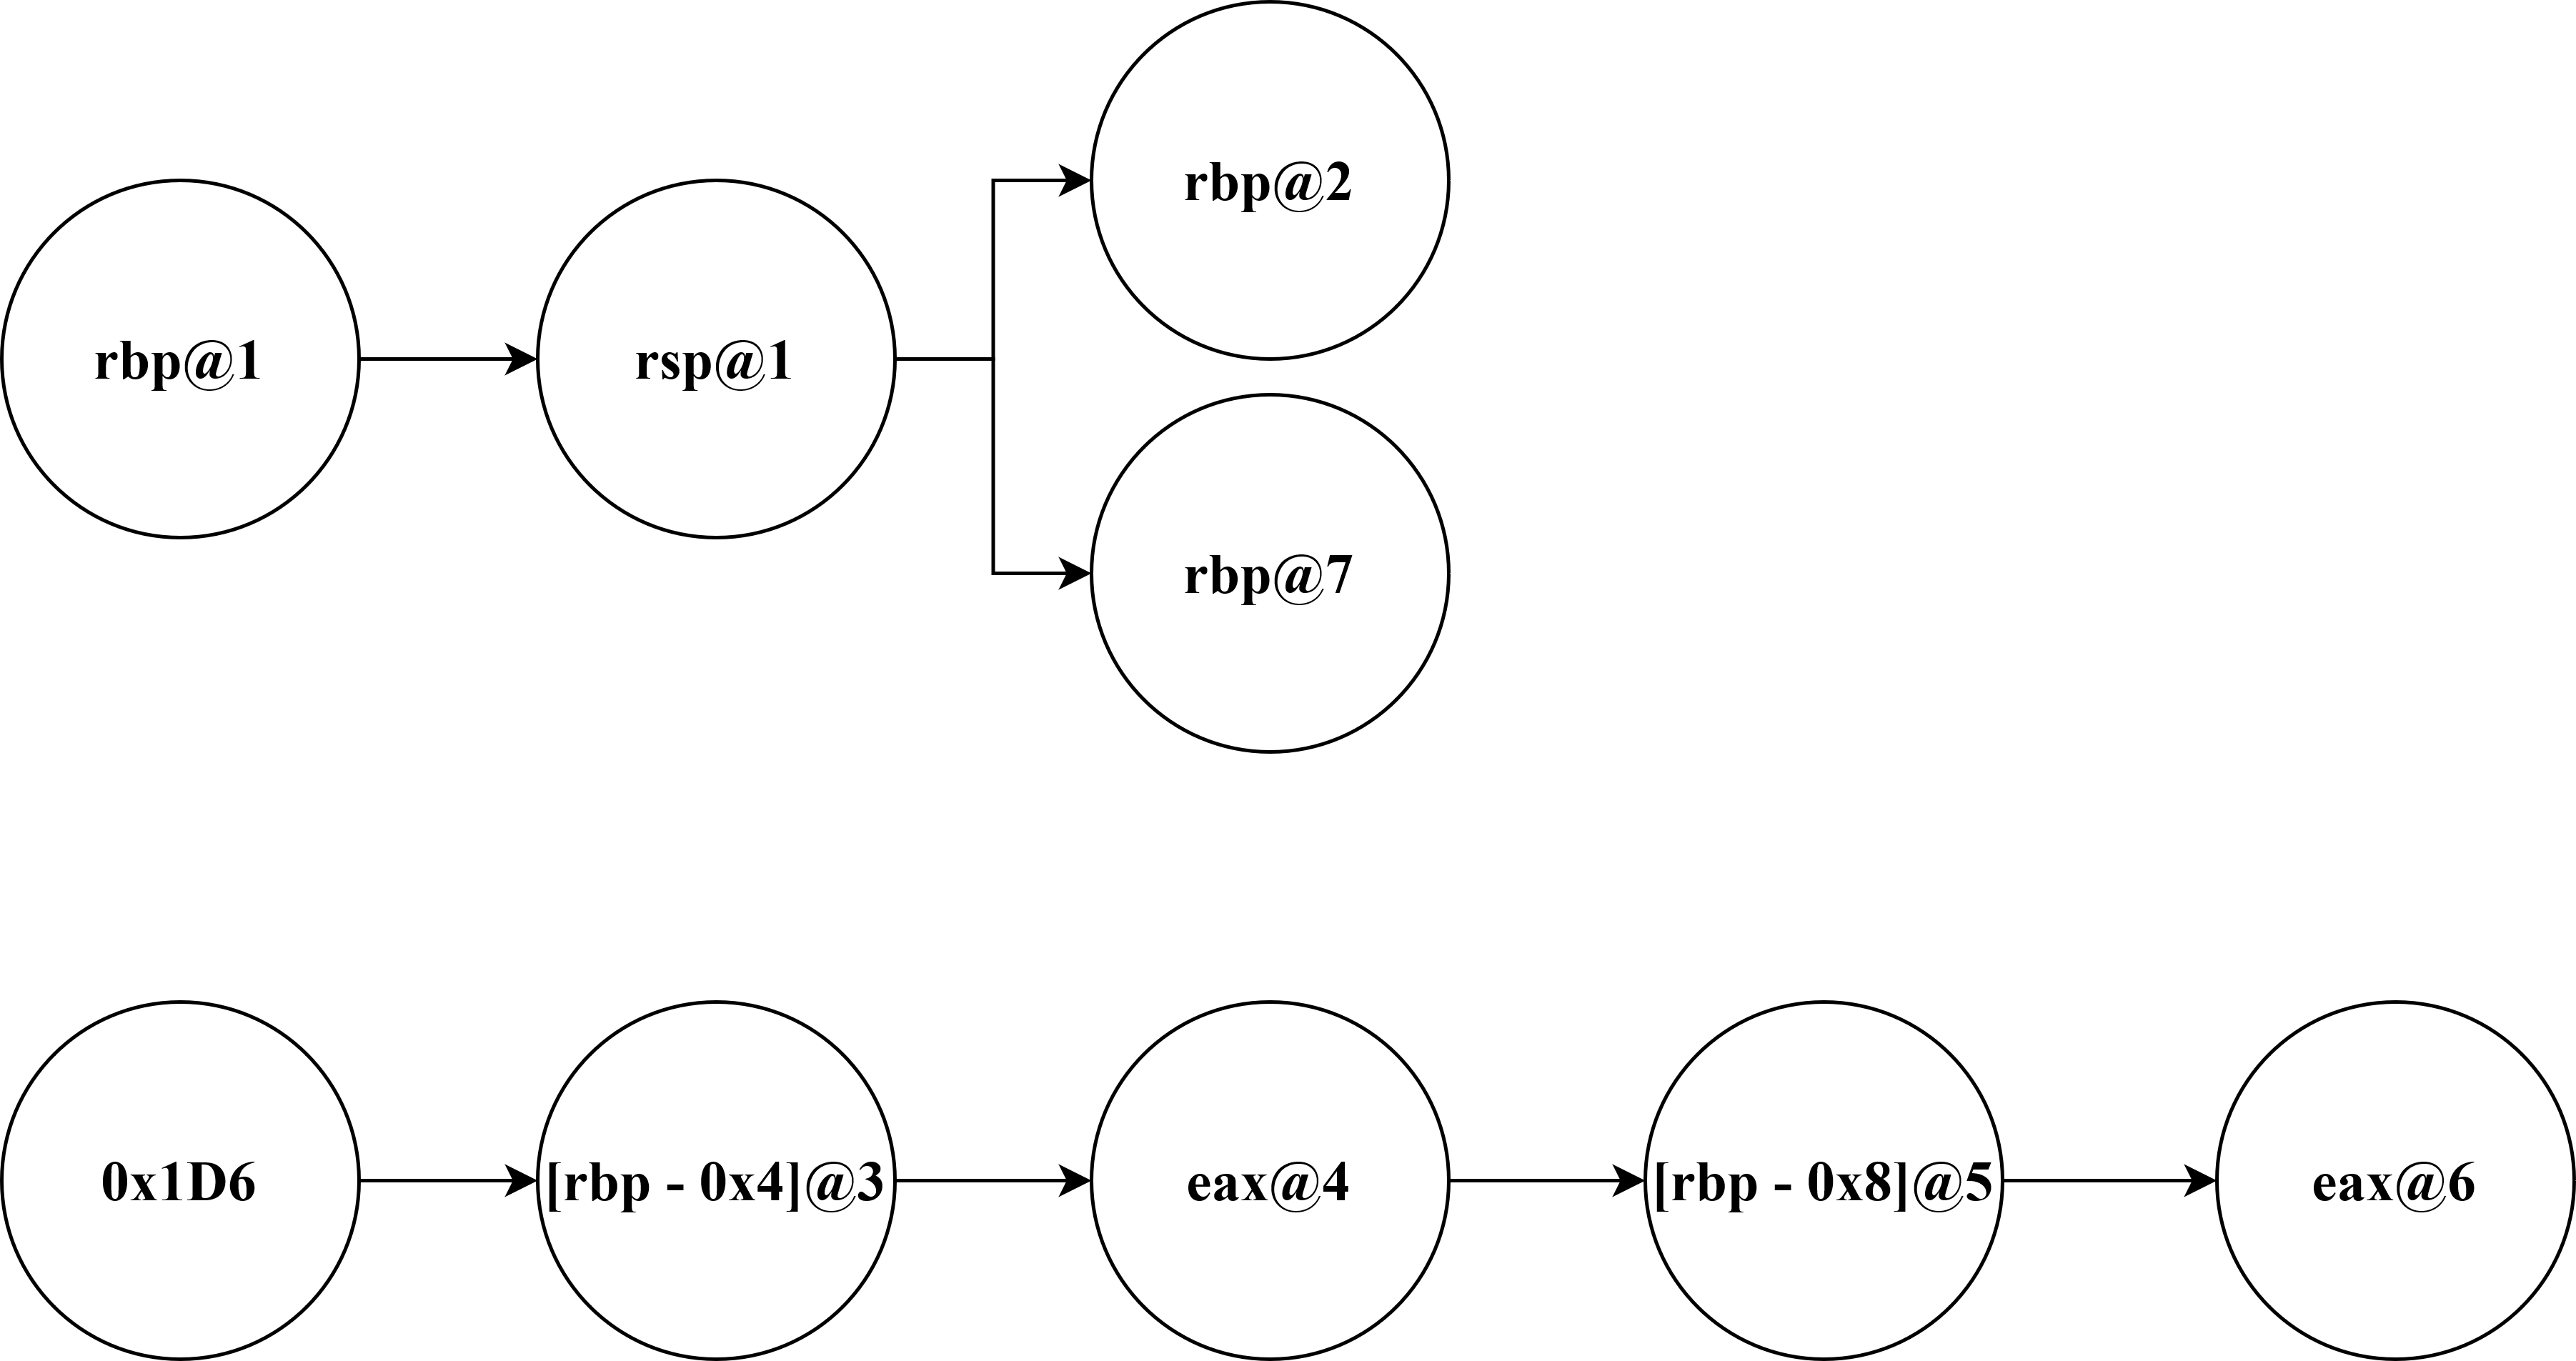
\includegraphics[width=0.8\linewidth]{images/ddg.png}
    \caption[DDG of Motivating Example]{DDG of motivating example, node names in form of location@address. Dependencies can be traced by following a node's edges backwards to view ancestors and forwards to view descendants.}
    \label{fig:motivddg}
\end{figure}

\section{Data Dependency Graph (DDG)}
A data dependency graph is a directed acyclic graph (DAG) that tracks all the data dependencies in a given execution trace. The data points, identified by their memory location and point of execution, serve as the graph’s nodes. The graph's edges originate from a source node and terminate at a dependent node. From any given node, one can follow the directed edges backwards to find the origin of a node’s value. By contrast, the edges leaving a node can be followed to find all dependent descendants in the data dependency graph. In the full dependency graph (Figure \ref{fig:motivddg}) of the code snippet provided in Figure \ref{fig:motiv}, the return value can be observed to have derived from a memory address ([rbp - 0x8]) which yielded its value from another address ([rbp - 0x4]) that had the constant written into it initially (with eax@4 being used to facilitate a memory to memory move in a RISC instruction set). While a toy example, it is evident that having a graphical representation of the flow of data within a more complicated program can prove invaluable to the binary analyst or software debugger.
\section{Intermediate Representation}
In compiler design, a source language can be translated into an arbitrary number of instruction sets. Thus, rather than developing optimizations for every unique target architecture, compilers utilize a middle-level, architecture-agnostic data structure instead \citep{grune2012modern, muchnick1997advanced, aho2003compilers}. This data structure is referred to as the intermediate representation (IR). The source code is translated into IR before optimizations are applied and later converted into the target architecture instruction set. Just as compilers require an intermediary language to apply universal optimizations to source code, so too do decompilers such as \code{angr}’s. Although, in the case of decompilers, the process entails converting an arbitrary number of instruction sets back into a higher-level universal language. The intermediate representation used by \code{angr} is borrowed from \code{Valgrind} and is called \code{VEX} \citep{vexir}. Rather than operating on machine code, which would require a tremendous amount of architecture-aware code to handle the many cross-architecture idiosyncrasies, the proposed analysis operates on \code{VEX} IR.
\include{relatedwork}
\chapter{DESIGN}
\begin{figure}[ht]
    \centering
    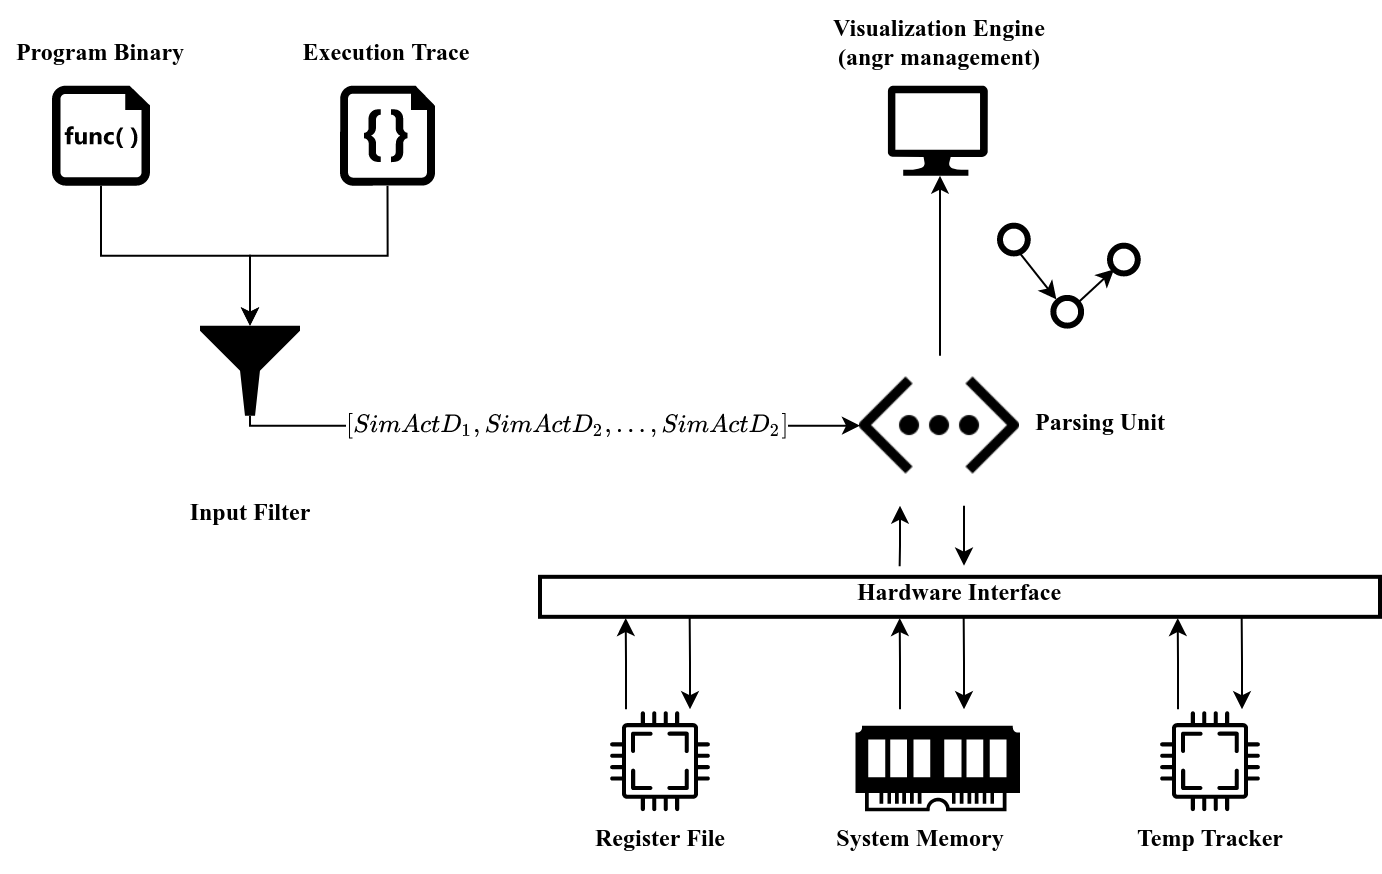
\includegraphics[width=0.8\linewidth]{images/design.png}
    \caption[Design Diagram]{Design diagram of proposed analysis.}
    \label{fig:design}
\end{figure}

The design goal of the proposed analysis is to ingest an arbitrary binary and execution trace and efficiently parse a representative data dependency graph for visualization. In order to develop this functionality, the design was split into the independent modules seen in Figure \ref{fig:design}.

\section{Input Filter}
This module is responsible for ingesting two critical files for data dependency graph generation: the program binary and the execution trace. The binary can be any executable file that the user would like to analyze while the execution trace must correspond to that binary. While execution trace generation was outside the scope of this thesis, the user could perform symbolic execution in \code{angr} upon the binary to generate it. This would typically involve creating the initial state at the first line of code that the user is interested in graphing and having the symbolic execution stop upon reaching the final line of code of interest. The resulting \code{SimState} must then be JSON encoded.

The input filter would then be responsible for decoding the execution trace to recover the underlying \code{SimState}. The only property of concern to this analysis within the \code{SimState} is its history, which contains an array of the read and write actions undertaken during symbolic execution. This array contains a series of \code{SimAction} instances, which may not all necessarily be concerned with the flow of data throughout the program's execution. The instances that belong to the \code{SimActionData} class are the only elements that concern data movement. Thus, this module will filter out all of the irrelevant elements from the history and output an array of the program's \code{SimActionDatas} in ascending order of the time in which they were taken.

\section{Parsing Unit}

\begin{figure}[hb]
    \centering
    
\includegraphics[width=0.8\maxwidth{\textwidth}]{cfg.png}
    \caption[Context Free Grammar of the Analysis' Language]{Context free grammar of the analysis' language. Designed to tightly mirror the aspects of \code{VEX IR} relevant to this analysis.}
    \label{fig:cfg}
\end{figure}

The parsing unit is the main module of the proposed analysis. 
I designed a context free grammar (Figure \ref{fig:cfg}) to capture the structure of the linear sequence of reads and writes ingested by the analysis. A recursive descent parser processes this sequence. This grammar follows the same structure of describing CPU actions that are taken by \code{VEX}. This design decision was driven by the fact that the grammar in question is relatively concise, and the code required to implement a recursive descent parser tightly mirrors the grammar \citep{redziejowski2007parsing}. Furthermore, the code that drives this analysis will need continued maintenance beyond the time frame of this thesis. Moreover, keeping the parser simpler and more readable, will make future contributions and improvements easier.

The terminals in the proposed context-free grammar  are used to represent the different categories of \code{SimActionData} that the analysis processes. As can be seen in the naming scheme of the terminals, a \code{SimActionData} is categorized based upon its action and type. The supported actions are WRITE and READ while the supported types are TMP, MEM, and REG. Although the MEM and REG types are straightforward, representing any operations that involve a memory address or register, the TMP type is not as readily apparent. TMP, short for temporary, operands can be viewed as variables as they are used to hold the result of intermediary steps in an operation. As an example, the AMD64 instruction \code{mov dword ptr [rbp – 0x4], 0x1d6} which moves the decimal value 470 into a memory offset from the base pointer, could be represented by the \code{SimActionDatas} presented in \ref{fig:tmp}. In this example, two temporary variables are used to hold the value of the base pointer register and the calculated offset from rbp to facilitate the memory write. 

\begin{figure}
    \centering
    
\includegraphics[width=0.8\maxwidth{\textwidth}]{tmp.png}
    \caption[Example of Temporary Operands in Angr]{Example of temporary operands in \code{angr}.}
    \label{fig:tmp}
\end{figure}

The largest unit that the analysis is concerned with is the block, with a program being a sequence of blocks. In \code{VEX}, a block is a collection of instructions with a single entrance and an unbounded number of exits. The end of a block is simply delineated by the \code{SimActionData} currently being parsed having a different block address from the next.

An instruction, while not being part of the \code{VEX} language, is incorporated into the analysis’ parser simply for readability. Rather than parsing the many statements that belong to a single block at a time, the statements belonging to a given instruction address are logically grouped. The end of an instruction is depicted by the \code{SimActionData} currently being parsed having a different instruction address from its successor. 

A statement is the smallest and most important unit of analysis, as \code{VEX} statements are what change state in the symbolic execution. A statement is parsed according to its type and action. It is during this portion of parsing where nodes in the data dependency graph are created and linked together.

The recursive descent parser is used to convert the provided sequence of \code{SimActionData} elements into a data dependency graph. The data dependency graph is then forwarded to the visualization engine for rendering a visualization to the screen.

\section{Hardware Interface}
This module serves as a supplementary module to the parsing unit, providing it with a memory of the read and write actions parsed thus far. This is imperative to have as, without tracking the reads and writes, it isn't possible to create edges between the nodes generated by the parser. The hardware interface facilitates the interactions between the parsing unit and the simulated register file, simulated system memory, and temporary tracker. The parsing unit can request to read from or write to a given register, variable, or memory address through the functionality it exposes.

In order to track the current state of all registers that the program moves data into and out of, an emulated register file is utilized to associate the register’s current value with its associated node in the graph. On a write to a register, the value and associated node are updated. On a read from a register, the current associated node is used as the value’s source for linking purposes. 

In order to track the current state of all memory addresses that the program reads and writes to, an emulated memory is also maintained. This works in the same manner as the register file. 

The temporary variable tracker is a per-block association of values with the current temporary node. This is reset at the end of a parsed block.

\section{Visualization Engine}
This module is responsible for ingesting the generated data dependency graph and visualizing it in an effective user interface for the binary analyst to peruse. This was accomplished through the creation of an \code{angr management} view.
\chapter{IMPLEMENTATION}
Data dependency generation is implemented as an \code{angr} analysis and is registered under the name ‘DataDep’. This allows the \code{angr} library user to access and utilize DDG functionalities through \code{project.analyses.DataDep()}. To maintain interoperability between DataDep and other \code{angr} analyses, the analysis outputs an instance of a NetworkX Digraph representing the generated DDG \citep{networkx}. The generated graph can then be further operated upon by the user or visualized using standard NetworkX visualization techniques \citep{networkxdraw}

In order to generate a DDG, the analysis must be provided a symbolic execution state which acts as a source of data moves performed by the program. This state is referred to as an “end-state”, as it provides a history containing all the reads and writes taken by the program up until a given endpoint. In \code{angr}, these simulated read and write actions are encapsulated in $SimActionDatas$. As far as \code{angr} is concerned, an action can be one of the types seen in Table \ref{table:types}.

\begin{table}
    \begin{center}
        \caption[Supported Action Types]{Supported Action Types.}
        \label{table:types}
        \begin{tabular}{ |c|c| }
        \hline
        \textbf{Type of Action} & \textbf{AMD64 Example} \\
        \hline
        A read from a `variable' & \code{mov rdx, rdi} (in terms of \code{rdi}) \\
        \hline
        A write to a `variable' & \code{mov rdx, rdi} (in terms of \code{rdx}) \\
        \hline
        A read from a memory address & \code{mov r9, [rax]} \\
        \hline
        A write to a memory address & \code{mov dword ptr [rax], 0xdeadbeef}) \\
        \hline
        \end{tabular}
    \end{center}
\end{table}

As naively ingesting an end state that captures all the reads and writes performed by a large program would result in a tremendous and unwieldy number of nodes for the user to parse through, the analysis supports a finer-grained approach by tailoring the graph to a portion of code of interest. This is accomplished by providing a symbolic execution state that begins its execution at the earliest point in time of concern and ends its execution on the instruction one beyond the latest point in time of concern. This “end-state” serves as the execution trace that must be provided along with the binary in question. The user may also optionally specify the block instructions or range of instruction addresses to include in the graph.

\section{Dependency Nodes}
The analysis operates on four distinct classes of nodes: memory, register, temporary, and constant. The first three types of nodes are used to represent a MEM, REG, and TMP \code{SimActionData}, respectively. The final nodal type, constant, is used to represent any untracked, literal value written or read from a \code{SimActionData}. As constants cannot, by definition, be dependent upon any other node. In other words, one cannot write to the decimal value 470. Thus, constants will always appear as the highest-level ancestors in a DDG. Each of these node types is represented by a corresponding class of nodes used by the analysis. The inheritance relationships between these classes, as seen in Figure \ref{fig:dep} is explained in greater detail below.

\begin{figure}
    \centering
    
\includegraphics[width=0.8\maxwidth{\textwidth}]{dep.png}
    \caption[UML Diagram of Dependency Node Class Inheritance]{UML diagram of dependency node class inheritance. All nodes in a generated data dependency graph are represented by the leaf classes in this figure, with all other classes being abstract.}
    \label{fig:dep}
\end{figure}


\subsection{Base Dependency Nodes}
The base dependency node class is abstract and serves as a template for what attributes its descendant classes must have. This class defines that, at a minimum, a node possesses a class type, instruction address, statement index, and action identifier. While the instruction address and statement index is straightforward, being the instruction of the address in which the dependency node resides and the index of the statement in that address respectively, the action warrants explanation. The action identifier is sourced directly from the node’s corresponding \code{SimActionData} and is a unique counter marking the occurrence of the given action in the entire program’s execution. 

\subsection{Constant Dependency Nodes}
The constant dependency nodes class is concrete and represented in a generated DDG. It is solely identified by its value.

\subsection{Memory Dependency Nodes}
The memory dependence nodes class is also concrete and represented in a generated DDG. In addition to the attributes that identify a base dependency node, a memory dependency node is further identified by its memory address. 

\subsection{Variable Dependency Nodes}
The variable dependency nodes class is abstract, serving as a common ancestor to temporary and register dependency nodes. While temporary and register nodes are different types of \code{SimActions}, both are identified by a register number and can be parsed without needing to be differentiated. 

\subsection{Temporary Dependency Nodes}
\label{section:tmp}
The temprorary dependency nodes class is concrete and represented in a generated DDG. While it adds no additional functionality to its base class, it is included in order to differentiate between register and temporary nodes for ease of filtering the graph for display. As the number of temporary nodes will be high for a given program, it is often beneficial to hide them in a generated DDG. 

\subsection{Register Dependency Nodes}
The register dependency nodes class is concrete and represented in a generated DDG. It exists to differentiate between register and temporary nodes for the reasons proposed in Section \ref{section:tmp}

\section{Generating and Tracking Nodes}
Based on the type and action of the \code{SimActionData} currently being parsed, different fields are pulled out of the action to create the respective dependency node. Upon creating a node for an action, the action is popped from the parsing queue and the node is added to the graph. The node is originally unconnected, as it has yet to be linked to the DDG.  

\section{Linking Nodes}
\begin{figure}
    \centering
    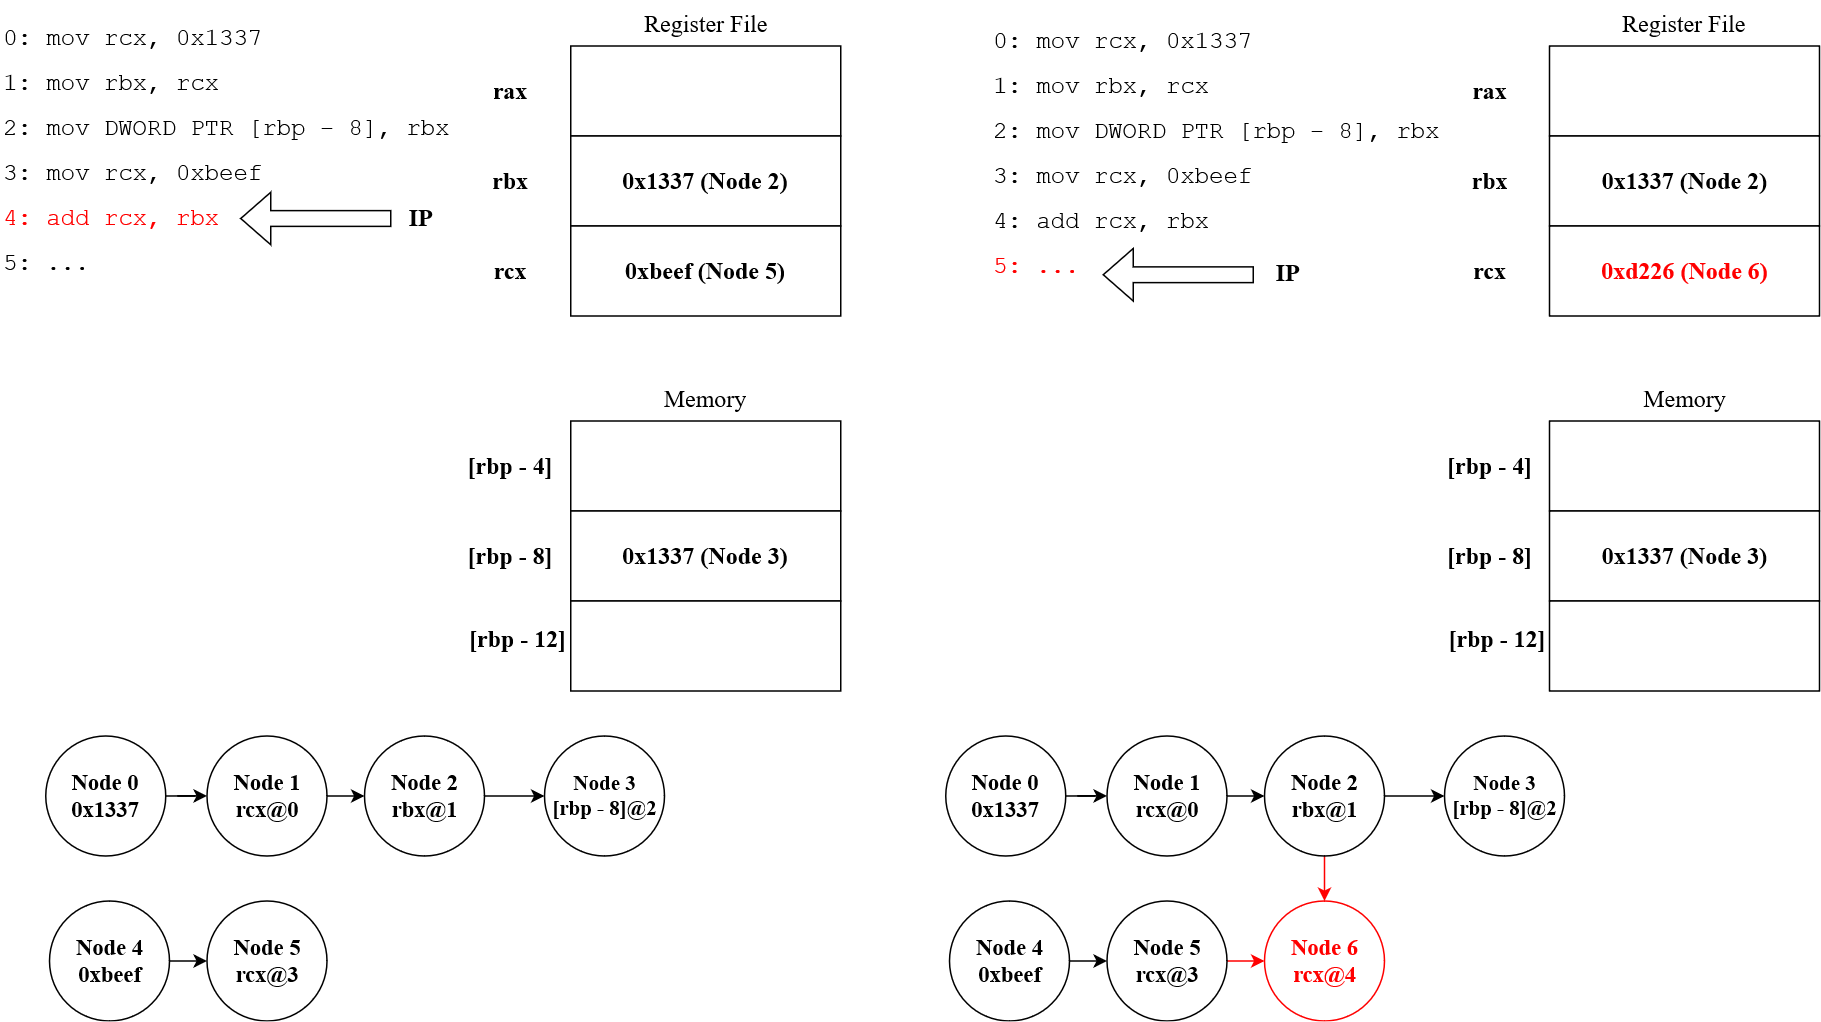
\includegraphics[width=1\maxwidth{\textwidth}]{state.png}
    \caption[Register File and Graph State Before and After Executing Instruction 4]{Register file and graph state before and after executing instruction 4. After executing the addition instruction, a new node for the destination operand is created and linked to the source operands. The register file for the destination operand is also updated to point to this new node.}
    \label{fig:link}
\end{figure}
The program in Figure \ref{fig:link} will be used as a motivating example to explain the linking process. The leftmost diagram gives an overview of the state of the register file, memory, and graph prior to the execution of instruction 4 and will serve as the state that is used to determine dependencies. As an add requires the CPU to read the value from the source operand and target operand, nodes 2 and 5, which are currently associated with \code{rbx} and \code{rcx}, respectively, will be located in the register file and tracked as data sources. Once the addition is calculated by the ALU, the value is then written back to the target operand (\code{rcx}). To facilitate this in the analysis, node 6 is created for \code{rcx} at this state and is linked to its two tracked source nodes as a dependency. As the next operation that utilizes \code{rcx} as an operand should be reliant upon the value of \code{rcx} post-addition, the register file for \code{rcx} is updated to point to node 6.

\section{Visualizing Nodes}
\begin{figure}
    \centering
    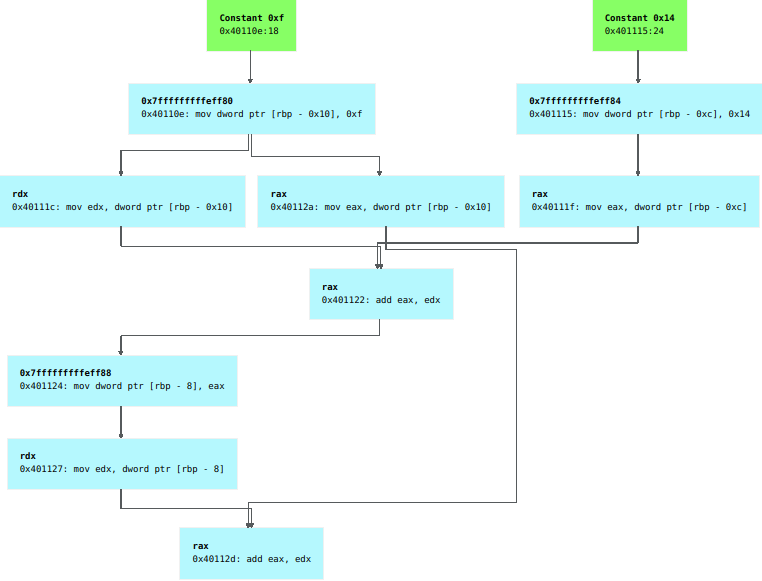
\includegraphics[width=0.6\maxwidth{\textwidth}]{viz.png}
    \caption[{Visualization of a Simple Data Dependency Graph}]{Visualization of a simple data dependency graph. This screenshot is of a subgraph that traces two subsequent additions.}
    \label{fig:viz}
\end{figure}

In addition to implementing the backend analysis for generating a data-dependency graph, its visualization was also within the scope of this thesis. This was accomplished through contribution to \code{angr management}, the official frontend for \code{angr}. An example visualization of a simple data dependency graph is depicted in Figure \ref{fig:viz}.

To improve the user experience, various features were implemented to aid the user in more quickly resolving the dependency of instructions with which they are concerned. For example, search functionality is available to jump through all nodes that match a provided name, instruction address, and/or value. Any of these fields can be omitted in the search, and thus will not be considered in node filtering. In addition to this feature, temporary nodes can be toggled on and off to prevent the screen from being cluttered with useless information when the temporary variables are not relevant to the analysis More importantly, however, the most relevant control is the generation of subgraphs. 

\subsection{Subgraphs}
 A subgraph can be generated from any given node in the data dependency graph. That is, the user can specify to trace the dependency of node X “forwards” and view all nodes that are ancestors of X or trace “backwards” and view all descendants of X. This feature is especially helpful in decreasing screen clutter, as the majority of nodes on a graph will not be relevant to a given dependency trace. 
\chapter{EVALUATION}
The goal of the user study is to determine the effectiveness of the data dependency graph analysis and its \code{angr management} visualization with respect to software debugging and binary analysis. In order to quantitatively and qualitatively determine its effectiveness, a user study was designed in which participants were tasked with solving a series of software debugging and binary analysis challenges. The experiment was split into three phases: introduction, challenge-solving, and survey. During the introduction phase, participants were given an overview of \code{angr management} and the views they were allowed to utilize during the experiment. The challenge-solving phase entailed the participants working through the challenges and answering a series of questions concerning each challenge. After all challenges were completed, the participant would then enter the survey phase where a series of survey questions were administered that captured the participant’s relevant background and overall perceptions of the experiment.

\section{Control vs Experimental Groups}
Participants were randomly divided into a control and experimental group as determined by a random session key that was used to de-identify user data. A control group was introduced as a means of measuring baseline performance in the challenge-solving phase in comparison to the results of the experiment group in order to gauge effectiveness. Those participants who were assigned to the control group were only provided an overview of \code{angr management}, while those who were assigned to the experimental group were provided an additional overview of the functionality of the data dependency graph view. During the challenge-solving phase, the experiment group was allowed to utilize the data dependency view as an aid in analyzing the challenge binary. This feature was disabled for the control group.

\section{Challenges}
In regards to experiment duration, three challenges were designed for this experiment: two focused on software debugging and one similar to traditional CTF challenges which focused on binary analysis more generally. In the subsequent sections the challenges are described in further detail.
\begin{itemize}
    \item $Median$: This software-debugging challenge finds the median of nine numbers by means of four successive calls to a median function. The first three calls were responsible for finding the median of the trisected sub-arrays, with the final call finding the median of the previous three results. Although, a logical comparison error in the median implementation causes the second call to the function to return an incorrect median, cascading to an incorrect result from the final call as well. The user was tasked with determining which call to median resulted in the bug and the nature of the bug. 
    \item $Follow$: This challenge was designed to emulate a traditional CTF challenge, with the correct input printing a flag. In order to determine the correct input, the participant would have to follow a data dependency maze, following the value 0x1337 as it moves from register \code{rbx} to register \code{rax} through a complicated series of register shuffling with many dead-ends. If the user-specified path was correct, the flag would be printed to standard output. The user was asked to provide details about what they attempted during the solving time, if they were able to solve the challenge, and what their inputs to the program were. 
    \item $Notes$: This software-debugging challenge asked the user to resolve a mock user bug report in a note-taking application. This binary allows the user to create, read, edit, and delete notes. However, a failure to check for the existence of a note before dereferencing it in the read functionality would cause a null-dereference and segmentation fault. The user was asked to identify the source of the bug and detail its nature.
\end{itemize}

\section{Framework}
In order to ease the burden inherent in installing \code{angr} and recording their own data, participants were provided a cloud-based system which enables interaction with a pre-configured virtual machine. After being provided a session key, the user would be able to navigate to the experiment’s domain and begin the experiment at the time of their choice. The framework would walk the participant through a sequence of pages that served as a guide for the user’s session. After getting consent from the user, he or she would be presented with a general introduction to the study. After navigating to the next page, a pre-configured virtual machine accessible via RDP would be cloned and powered on for the user to solve the challenges on. This framework provided a reliable means of recording the user’s progress on the virtual machine and precise timestamps of how long each challenge took each user.  While the system pre-dates the experiment, various customizations were made in order to protect user data and introduce randomization. 

Randomness was key to eliminating bias and uncontrolled variables in this experiment. First, participants were randomly assigned to the control group, unable to use the DDG, or experiment group. The former enabled the experiment to have a measurable baseline. Secondly, the order of challenges was randomized per participant to eliminate the impact of progressive learning and fatigue on the later challenges. To achieve this randomness, the user’s unique session key was used as the seed to a random number generator that decided these factors. Once the sequence was shuffled, the survey pages associated with each challenge were dynamically shuffled to match the new order. While the participation website was easily randomized, the challenge of syncing \code{angr management} on the virtual machine to utilize the same randomness proved more complex.

\section{Custom \code{Angr} Wrapper}
The design of the experiment required modifications to \code{angr management}, namely support for restricting access to views and loading binaries in a pre-determined sequence. For the sake of this experiment, the views in Table \ref{table:views} were permitted.
\begin{table}
    \begin{center}
        \caption[Permitted Views]{Permitted Views.}
        \label{table:views}
        \begin{tabular}{ |c|c| }
        \hline
        \textbf{Control} & \textbf{Experimental} \\
        \hline
        Functions & Functions \\
        \hline
        Disassembly & Disassembly \\
        \hline
        Hex & Hex \\
        \hline
        Strings & Strings \\
        \hline
        Interaction & Interaction \\
        \hline
        Console & Console \\
        \hline
        Log & Log \\
        \hline
        & Data Dependency \\
        \hline
        \end{tabular}
    \end{center}
\end{table}
Noticeable omissions include decompilation and symbolic execution. These were removed to address the inherent challenge of designing challenges for a ten-minute time frame. They must be simple enough to be solved within the time frame but complicated enough to warrant analysis. These challenges would be trivial with access to decompilation and symbolic execution. If included, the experiment would be invalidated. Rather, pitting data dependency against disassembly view, which it seeks to complement, makes more sense for the scope of this project. 

The greater challenge occurred when syncing the order of loaded binaries and trace files with the web server. As some form of communication of the randomly generated group membership and challenge order needed to be transmitted from the server to the virtual machine, a binary-encoded JSON file was written to the virtual machine upon creation utilizing the \code{VirtualBox} command execution functionality. When the customized \code{angr} wrapper was launched by the participant, it would first check for this file and reorient the order in which it loads binaries to sync with the server.

\section{Survey}
After completion of each challenge and its associated questionnaire, the user was asked to provide more general feedback by means of a final survey. The participants were asked questions pertaining to their experience in software debugging and vulnerability analysis, their comfort with \code{angr management}, and their overall understanding of the challenges provided. While these questions were asked of all participants, further questions were asked dependent upon group membership. For those users in the control group, an example data dependency graph screenshot was provided. Questions about the perceived usefulness and clarity of the ‘hypothetical’ view accompanied the screenshot. Contrarily, users in the experiment group were asked to rate data dependency graph view in terms of its usefulness and clarity. Additionally, a free-form further feedback field was provided to ascertain the user’s thoughts regarding future improvements that could be made to the view.

\section{Collected Data}
In addition to the user’s responses to the challenge questionnaires and survey, the time a user took to complete each challenge was recorded. This data will be used to quantify a performance delta between control and experiment groups in terms of challenge-solving speed. Lastly, the user’s virtual machine session was video recorded as a means of verifying user’s participation and to resolve any possible bugs or crashes should they have occurred. No personally identifiable information was tracked or stored in the server’s database. Instead of utilizing a name or email, data is tethered to a session by the random, unique session key provided to each user.  
\include{results}
\chapter{DISCUSSION}
\section{Lessons Learned}
Throughout the course of this thesis, an abundance of lessons were learned with respect to designing a user interface tailored to the user’s experience and a user study able to capture the efficacy of the DDG. The lessons outlined in this section will serve as the motivation for potential future work.  

The results of the survey reveal that a sizable portion of the study-base found the user interface confusing or lacking in desired functionality. Largely, the suggested functional additions and improvements promote better interaction between the user and the generated data dependency graph. Asking the user for a trace file and displaying the entire data dependency graph is not in line with the user’s expectations or interests. Rather than displaying the entire graph at once, with all the nodes in the provided trace file’s history and expecting the user to utilize the search functionality to navigate, it would be better to allow the user to filter down the graph prior to displaying it. The analysis’ backend currently supports more fine-grained approaches to DDG generation but are not reflected by endpoints in the user interface. Possible improvements will be described in the future work section.

As for the design of the user study, the use of randomization had its drawbacks. While instrumental in eliminating the effects of fatigue and progressive learning, the randomization of challenge order without respect to challenge difficulty proved problematic. While the effect of progressive learning was eliminated, this proved counter-intuitive when the user was randomly assigned one of the more difficult challenges first. In their feedback, some participants noted that they would have appreciated starting with one of the later challenges first to better learn data dependency view prior to applying it to a more difficult challenge. A possible solution that would still eliminate the effect of progressive learning but also resolve the issue of users facing more difficult challenges first would be to have each challenge scale its difficulty to correlate to its randomized order in order to maintain an easy $\xrightarrow[]{}$ medium $\xrightarrow[]{}$ hard progression.

In addition to the effects inherent in randomization, whichever challenge the user was initially assigned would have a completion time swayed by factors excluding difficulty. As many participants did not have prior experience with \code{angr management}, asking them to learn the basics of interacting with the framework, the novel view, and solving a challenge all at once had a definite sway on the time it takes to complete the first task. 

After analyzing the results, the importance of wording in questions and objectivity were understood to be paramount. Questions concerning the user's self-perceived skill level was not statistically tied to results, and thus those types of questions proved useless. Furthermore, the wording of the median questions proved confusing to some participants. This required more lenient grading that took into account the user's free-form feedback as opposed to grading their multiple choice answers exclusively. 

As evidenced by feedback asking for functionality that was already explained on the introductory page, the medium by which the introductory lesson was delivered was not effective. Research has shown that product manuals are not an effective means of conveying information to users. Most people do not read instruction manuals and will utilize a fraction of a product's features and functionality \citep{blackler2016life}. Rather than presenting the introduction as a static webpage, a video would have been more engaging and provided users with a clearer demonstration of the features at their disposal. The decision to convey feature implementation had a serious negative effect on user perception of the data dependency view, with users requesting zoom functionality, subgraph functionality, search functionality, and node highlighting. All of these features were explained in the introduction. 

The largest lesson learned was the downsides of deploying this experiment on a cloud-based framework. While the use of a cloud-based solution allowed for participants from the wider cybersecurity community as well as more flexibility with the participant’s schedules, many users reported latency as a discomfort during the challenge-solving phase. While already being a network-intensive protocol, RDP becomes far more unusable with distance. Many interested participants from Europe and Asia were unable to complete the experiment due to the unbearable latency. The latency inherent to RDP even had a negative impact on user feedback in regards to the views comprehensibility. As evident from the free-form feedback, two participants found the view confusing due to the lag they encountered while using data dependency view. This will have had an effect on the data, despite being an independent variable. Future studies would have to weigh this consideration into account when considering experiment deployment methods.
In addition to relying on a server to conduct this experiment, participation was very much at the mercy of the server’s uptime and performance. Early in the user study, the server suffered from thrashing and would shut down under high load. Prior to this error being resolved, various participants would either have to have their results thrown out or were discouraged from continuing. Thus, if a cloud-based solution were to be utilized in a future user study, more servers would need to be deployed globally, clustered by participant locality. Having multiple servers would also serve as fault-tolerance, with one malfunctioning server offloading its work onto its peers to prevent interruption of participation.

\section{Future Work}
As evidenced by the feedback received and discussed in the lessons learned, work must be done to improve the user interface. Possible improvements and reworks, as aggregated from participant feedback, will now be described in greater detail. 

About 1/5 of users reported a desire for a more cohesive experience when using data dependency graph. Rather than loading a trace file for the current binary, these users stated they would prefer the option to right-click the constants or instructions in the disassembly view that they would like to generate a data dependency graph of. The current implementation could easily be pivoted to accommodate this modality of interaction. A symbolic execution state could be initialized at the earliest instruction in the user-specified selection and allowed to run, with a find target of the end instruction. Should there be a path that exists, the state at the end of symbolic execution could be passed to the data dependency analysis.

While the aforementioned solution will work, symbolic execution is an expensive operation. If the user were to only use data dependency on one or two instruction subsets during their analysis, then no further optimizations are necessary. Although, should the user wish to generate many DDGs, the lag between the start of the task and the generation of the view would be an annoyance. A possible solution would be to move the data dependency generation to a background thread that, upon completion of the underlying analysis, emits a Qt signal to inform the main thread that it can now generate the view. While the same amount of time would be required to generate the view, the UI would not be locked until completion and the user would be free to continue their analysis elsewhere.  

Another possible optimization could see the generation of a DDG being queued upon the user’s first request to see one. Regardless of the instruction subset requested, an initial request could see the data dependency analysis being dispatched in a background thread for the entire program-space. While the first data dependency graph requested would be slower, all subsequent calls could just utilize the subgraph functionality and be near instantaneous. Although, this solution has many trade-offs: increased computation that may go unutilized, more utilization of RAM to store the larger Digraph, and some binaries being far too large to warrant a DDG being generated for the entire program-space.

User feedback suggested that the current user interface provides a jarring experience when attempting to manually follow a dependency in the graph. For one, the scrolling speed resulted in users losing their place in the graph. Additionally, users reported a desire for color-coding certain paths branching out of a node to make manual tracing more feasible. This problem is compounded by the clutter produced by the arrows in the graph which should also be addressed.

The last category of improvements suggested by the users was improvements to searching. The search panel should allow users to specify if they would like to search within the current sub-graph or within the entire data dependency graph, as a few users voiced their desire for this functionality. Users also requested the ability to search for instructions using regex. 

Future work on data dependency graph should be focused on bridging the divide between data dependency graph and disassembly view / decompilation view. The ability to more quickly switch between the control flow graph and the data dependency would address the majority of feature requests from the participant pool.

Another promising vein of research for inclusion in data dependency graph is the application of taint analysis in deciding how graphs should be generated \citep{clause2007dytan, newsome2005dynamic, zhu2015dytaint}. The application of taint analysis could make data dependency graph more relevant in the realm of vulnerability analysis, as a correlation could not be established for the view proposed in this experiment. With the ability to specify sources (user-controllable origins of data) and sinks (potentially vulnerable instructions or functions) a data dependency graph could be generated that shows any existing connections between the source and the sinks. With the ability to trace forwards from the source to a sink or backwards from a sink to the source, the user would be presented with the series of checks and input restrictions required to exploit the vulnerable code in question. Furthermore, breadth-first search could be employed to find the shortest path from a given source to a given sink if multiple dependency paths exist (to make exploitation easier). Presenting the shortest path as opposed to the entire data dependency graph would also help prevent overloading the user with a massive dependency tree.
\chapter{CONCLUSION}
Two contributions were made through this paper. First, a data dependency graph analysis was introduced as a new means of analyzing binaries in the \code{angr} ecosystem. By employing a recursive-descent parser and a simulated register file and dedicated memory, the analysis is able to track dependencies between data regions throughout a program's execution. The subset of instructions analyzed can be altered through fine-grained controls that allow the user to specify a subset of executed instructions for graph generation. This data dependency graph can also be visualized through a custom \code{angr management} data dependency view.

Secondly, the efficacy of this view was tested through a user study that utilized a customized \code{angr} wrapper and a cloud-based deployment framework. In the experiment, users were split into a control and experimental group and were asked to solve a series of software-debugging and more generalized binary analysis challenges. The results showed an overall increase in the number of challenges correctly solved amongst the experimental group, with a statistically significant increase involving the challenge concerning data dependencies. As for time to solve, participants in the experimental group were able to solve the challenges much faster than their peers in the control group. No statistical significance could be attributed to this observation. Users perceived the view to be incredibly functional, but found its comprehensibility challenging. Based off of user feedback, a numerous amount of lessons learned were proposed with possible future work detailed.

The implementation of data dependency graph in its current state, while showing promising results in its niche, is just the beginning of the possible impact this view could have on binary analysis speed and accuracy. Should the suggestions posed in the future work be adopted, the view could see much more impressive results in future user studies. It is hoped that the user study design proposed in this paper should serve as a template for any future studies in this vein in order to continue to enrich the suite of tools available to the software debugger and binary analyst of the future.
%-----------------------back matter
{\singlespace
% Making the references a "part" rather than a chapter gets it indented at
% level -1 according to the chart: top of page 4 of the document at
% ftp://tug.ctan.org/pub/tex-archive/macros/latex/contrib/tocloft/tocloft.pdf

\pagestyle{tocheader}
\addcontentsline{toc}{part}{REFERENCES}
\bibliographystyle{asudis}
\bibliography{dis}}
\renewcommand{\chaptername}{APPENDIX}
\addtocontents{toc}{APPENDIX \par}
\appendix
\addtocontents{toc}{\protect\setcounter{tocdepth}{0}}
\chapter{RECRUITMENT ADVERTISEMENT}
\newpage
In order to recruit participants from the various academic and cybersecurity Discord servers, the following message was sent out:
Have you taken ASU’s CSE 365, CSE 466, or CSE 545 or do you have a background in reverse engineering, debugging, and exploiting binaries? If you answered “yes” to either of these questions, you are invited to participate in a research study conducted by Arizona State University! You will be asked to solve various challenges using a tool called angr management in order to research the effectiveness of new features on the platform. Prior experience with angr management is not necessary. The research study is approximately 1.75 hours (100 minutes) and can be taken at your time of choice. Your participation will be rewarded with a \$50 Amazon gift card upon completion. For more information, contact <contact details>. Participation in this study is voluntary.

\chapter{SURVEY QUESTIONS}
\newpage
\section{Median}
\begin{enumerate}
    \item Have you seen this challenge before?
    \begin{itemize}
        \item Yes
        \item No
        \item I prefer not to answer
    \end{itemize}
    \item Briefly describe what you did during this challenge (bullet point explanation is acceptable):
    \begin{itemize}
        \item Free form response
    \end{itemize}
    \item Were you able to identify the source of the bug?
    \begin{itemize}
        \item Yes
        \item No
        \item I prefer not to answer
    \end{itemize}
    \item After which function call to middle does the error originate?
    \begin{itemize}
        \item First
        \item Second
        \item Third
        \item Fourth
        \item I do not know
        \item I prefer not to answer
    \end{itemize}
    \item Which of the following best describes the nature of the bug?
    \begin{itemize}
        \item Memory corruption
        \item Signed comparison bug
        \item Logical error
        \item Integer overflow
        \item I do not know
        \item I prefer not to answer
    \end{itemize}
    \item If possible, briefly describe the cause of the bug.
    \begin{itemize}
        \item Free form response
    \end{itemize}
\end{enumerate}

\section{Follow}
\begin{enumerate}
    \item Have you seen this challenge before?
    \begin{itemize}
        \item Yes
        \item No
        \item I prefer not to answer
    \end{itemize}
    \item Briefly describe what you did during this challenge (bullet point explanation is acceptable):
    \begin{itemize}
        \item Free form response
    \end{itemize}
    \item Were you able to solve the challenge?
    \begin{itemize}
        \item Yes
        \item No
        \item I prefer not to answer
    \end{itemize}
    \item What input(s) did you provide to solve this challenge?.
    \begin{itemize}
        \item Free form response
    \end{itemize}
\end{enumerate}

\section{Notes}
\begin{enumerate}
    \item Have you seen this challenge before?
    \begin{itemize}
        \item Yes
        \item No
        \item I prefer not to answer
    \end{itemize}
    \item Briefly describe what you did during this challenge (bullet point explanation is acceptable):
    \begin{itemize}
        \item Free form response
    \end{itemize}
    \item Were you able to identify the source of the bug?
    \begin{itemize}
        \item Yes
        \item No
        \item I prefer not to answer
    \end{itemize}
    \item In which function call does the bug emerge?
    \begin{itemize}
        \item delete\_note
        \item read\_note
        \item edit\_note
        \item create\_note
        \item I do not know
        \item I prefer not to answer
    \end{itemize}
    \item Which of the following best describes the nature of the bug?
    \begin{itemize}
        \item Uninitialized variable
        \item Signed comparison bug
        \item Syntax error
        \item Null dereference
        \item I do not know
        \item I prefer not to answer
    \end{itemize}
    \item If possible, briefly describe the cause of the bug.
    \begin{itemize}
        \item Free form response
    \end{itemize}
\end{enumerate}

\section{End Survey}
\subsection{Control}
 \begin{figure}[!hb]
        \centering
        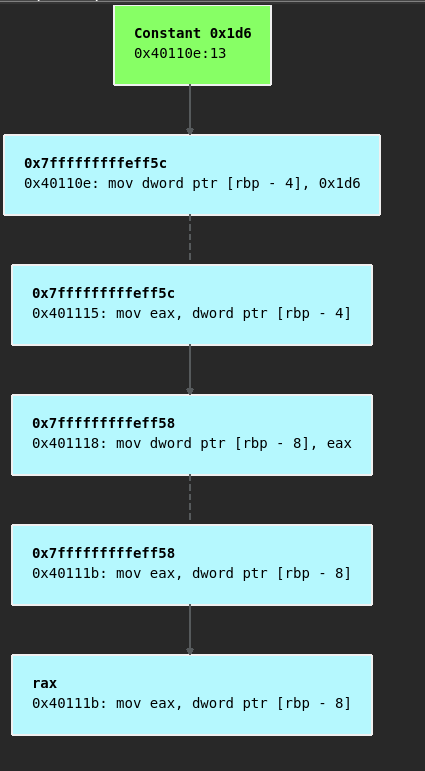
\includegraphics[scale=0.4]{images/surveyddg.png}
        \caption{Control group hypothetical data dependency view screenshot}
        \label{fig:surveyddg}
\end{figure}
\begin{enumerate}
    \item How many years experience do you have in software debugging?
    \begin{itemize}
        \item None
        \item Less than 1 year
        \item 1 year
        \item 2 years
        \item 2+ years
        \item I prefer not to answer
    \end{itemize}
    \item How many years experience do you have in vulnerability analysis?
    \begin{itemize}
        \item None
        \item Less than 1 year
        \item 1 year
        \item 2 years
        \item 2+ years
        \item I prefer not to answer
    \end{itemize}
    \item What is your perceived software debugging skill level?
    \begin{itemize}
        \item Novice
        \item Beginner
        \item Competent
        \item Proficient
        \item Expert
        \item I prefer not to answer
    \end{itemize}
    \item What is your perceived vulnerability analysis skill level?
    \begin{itemize}
        \item Novice
        \item Beginner
        \item Competent
        \item Proficient
        \item Expert
        \item I prefer not to answer
    \end{itemize}
    \item Have you used angr management before your participation today?
    \begin{itemize}
        \item Yes
        \item No
        \item I prefer not to answer
    \end{itemize}
    \item What is your perceived comfort level with angr management?
    \begin{itemize}
        \item Novice
        \item Beginner
        \item Competent
        \item Proficient
        \item Expert
        \item I prefer not to answer
    \end{itemize}
    \item I am sure that I correctly understood what the code of each challenge does
    \begin{itemize}
        \item Strongly Disagree
        \item Disagree
        \item Neutral
        \item Agree
        \item Strongly Agree
        \item I prefer not to answer
    \end{itemize}
    \item I found it difficult to understand these challenges
    \begin{itemize}
        \item Strongly Disagree
        \item Disagree
        \item Neutral
        \item Agree
        \item Strongly Agree
        \item I prefer not to answer
    \end{itemize}
    \item Disassembly view provided adequate information to solve these challenges
    \begin{itemize}
        \item Strongly Disagree
        \item Disagree
        \item Neutral
        \item Agree
        \item Strongly Agree
        \item I prefer not to answer
    \end{itemize}
    \item A data dependency graph view like in the image below (Figure \ref{fig:surveyddg})  would have been helpful
    \begin{itemize}
        \item Strongly Disagree
        \item Disagree
        \item Neutral
        \item Agree
        \item Strongly Agree
        \item I prefer not to answer
    \end{itemize}
    \item This view in the image below (Figure \ref{fig:surveyddg}) seems confusing and unnecessary
    \begin{itemize}
        \item Strongly Disagree
        \item Disagree
        \item Neutral
        \item Agree
        \item Strongly Agree
        \item I prefer not to answer
    \end{itemize}
\end{enumerate}


\subsection{Experiment}
\begin{enumerate}
    \item How many years experience do you have in software debugging?
    \begin{itemize}
        \item None
        \item Less than 1 year
        \item 1 year
        \item 2 years
        \item 2+ years
        \item I prefer not to answer
    \end{itemize}
    \item How many years experience do you have in vulnerability analysis?
    \begin{itemize}
        \item None
        \item Less than 1 year
        \item 1 year
        \item 2 years
        \item 2+ years
        \item I prefer not to answer
    \end{itemize}
    \item What is your perceived software debugging skill level?
    \begin{itemize}
        \item Novice
        \item Beginner
        \item Competent
        \item Proficient
        \item Expert
        \item I prefer not to answer
    \end{itemize}
    \item What is your perceived vulnerability analysis skill level?
    \begin{itemize}
        \item Novice
        \item Beginner
        \item Competent
        \item Proficient
        \item Expert
        \item I prefer not to answer
    \end{itemize}
    \item Have you used angr management before your participation today?
    \begin{itemize}
        \item Yes
        \item No
        \item I prefer not to answer
    \end{itemize}
    \item What is your perceived comfort level with angr management?
    \begin{itemize}
        \item Novice
        \item Beginner
        \item Competent
        \item Proficient
        \item Expert
        \item I prefer not to answer
    \end{itemize}
    \item I am sure that I correctly understood what the code of each challenge does
    \begin{itemize}
        \item Strongly Disagree
        \item Disagree
        \item Neutral
        \item Agree
        \item Strongly Agree
        \item I prefer not to answer
    \end{itemize}
    \item I saw no need to use data dependency view to solve these challenges
    \begin{itemize}
        \item Strongly Disagree
        \item Disagree
        \item Neutral
        \item Agree
        \item Strongly Agree
        \item I prefer not to answer
    \end{itemize}
    \item Data dependency view aided in understanding the challenges
    \begin{itemize}
        \item Strongly Disagree
        \item Disagree
        \item Neutral
        \item Agree
        \item Strongly Agree
        \item I prefer not to answer
    \end{itemize}
    \item Data dependency view is lacking in valuable information
    \begin{itemize}
        \item Strongly Disagree
        \item Disagree
        \item Neutral
        \item Agree
        \item Strongly Agree
        \item I prefer not to answer
    \end{itemize}
    \item I find data dependency view useful
    \begin{itemize}
        \item Strongly Disagree
        \item Disagree
        \item Neutral
        \item Agree
        \item Strongly Agree
        \item I prefer not to answer
    \end{itemize}
    \item Data dependency view is redundant and unnecessary
    \begin{itemize}
        \item Strongly Disagree
        \item Disagree
        \item Neutral
        \item Agree
        \item Strongly Agree
        \item I prefer not to answer
    \end{itemize}
    \item Data dependency view was clear and easy to understand
    \begin{itemize}
        \item Strongly Disagree
        \item Disagree
        \item Neutral
        \item Agree
        \item Strongly Agree
        \item I prefer not to answer
    \end{itemize}
    \item Data dependency view confused me
    \begin{itemize}
        \item Strongly Disagree
        \item Disagree
        \item Neutral
        \item Agree
        \item Strongly Agree
        \item I prefer not to answer
    \end{itemize}
    \item If any, what improvements could be made to make data dependency view more user friendly?
    \begin{itemize}
        \item Free form response
    \end{itemize}
\end{enumerate}
\include{vita}
\end{document}